%# -*- coding: utf-8 -*-
% !TEX encoding = UTF-8 Unicode
\RequirePackage{fixltx2e}
\documentclass[aps,pre,12pt,preprint,onecolumn,showpacs,showkeys,UTF8]{revtex4-1}
\usepackage{ctex}
\usepackage{setspace,dcolumn}
\usepackage{subfigure}
\usepackage{graphicx,psfrag,epsfig}
\usepackage[font=small,format=plain,labelfont=bf,textfont=it,justification=raggedright,singlelinecheck=false]{caption}
\usepackage{amsmath,amsfonts,amssymb,amsthm,bm,upgreek}
\usepackage{geometry}
\usepackage[mathscr]{eucal}
\usepackage{titlesec}
\titleformat{\section}{\bf\fangsong\zihao{4}}{\thesection}{0.75em}{}
\geometry{top=2.54cm,bottom=2.54cm,left=3cm,right=3cm}
\renewcommand\appendixname{附录}
\renewcommand\abstractname{}%摘要
\renewcommand\tablename{表}
\renewcommand\figurename{图}
\makeatletter
\def\@keys@name{\songti\zihao{-4}{\bf 关键词:}}
\def\Received@name{\zihao{-5}{接收} }
\def\Revised@name{\zihao{-5}{修订} }
\def\Accepted@name{\zihao{-5}{采纳} }
\def\Published@name{\zihao{-4}{发表} }
\makeatother
\linespread{1.6}
\renewcommand{\labelenumi}{\alph{enumi}.}
\leftmargini=20mm

\begin{document}

\title{\bf\heiti\zihao{3}电子自旋共振\vspace{15mm}}
\author{\fangsong 乔颢\vspace{2mm}}
\affiliation{\songti\zihao{-4}北京大学物理学院2011级2班~~~~学号:1100011354 \vspace{2mm}}
\keywords{电子自旋共振,微波,共振吸收,DPPH}
\email{1993422qsh@gmail.com; 18600200672}
\begin{abstract}
	\vspace{10mm}
	\begin{spacing}{1.5}
		\songti\zihao{-4}
		本次实验利用微波系统探测研究了二苯基——苦基肼基(DPPH)在外加磁场的情况下发生的顺磁共振现象,并且测量得到了研究对象的朗德因子,旋磁比以及驰豫时间的具体数值。实验结果比较好的符合了理论的预测,取得了预期的结果。
	\end{spacing}
\end{abstract}

\maketitle

\section{引言}
电子自旋共振(ESR)或者说电子顺磁共振(EPR)是指在含有未成对电子的原子、离子或者分子的顺磁性物质,在稳恒磁场的作用下原始能级劈裂,对合适的微波能量发生的能级间的共振跃迁吸收现象。如果共振仅仅涉及物质中的电子则被称为电子的自旋共振,而在一般情况下,电子的轨道磁矩不可忽略,所以被称作电子的顺磁共振。

电子顺磁共振通过观测研究对象的共振波谱,可以了解这些物质中未成对电子的电子状态以及其周围环境方面的信息。同时由于这种方法并不改变或者破坏研究对象本身的性质,因而对于那些寿命短,化学性质不稳定的分子或者自由基等的研究有着显著的作用。所以自1945年发现这个现象以来,顺磁共振已经在物理学,化学等领域中取得了广泛的应用\cite{Book}。

这个实验目的是利用微波系统和一系列的微波器件对DPPH自由基的电子自旋共振进行观测和测量,并与理论给出的数值进行验证。从实验的结果来看,实验数据基本上支持了理论给出的预测结果。

\section{实验}
\subsection{实验原理}
按照经典的理论,原子中的电子既有轨道运动,又有自旋运动。对于单电子院子,电子轨道角动量和自旋角动量合成为电子的总角动量。有电子的总磁矩也满足:
\begin{equation}
	\bm{\mu_j}=-g_j\frac{e}{2m_e}\bm{P_j}
\end{equation}
式中$\bm{P_j}$为电子总角动量,$e$为电子电荷,$m_e$为电子质量,$g_j$则为朗德因子。其数值满足以下关系:
\begin{equation}
	\mu_j=-g_j\frac{e}{2m_e}P_j	
\end{equation}
其中:
$$P_j=\sqrt{j(j+1)}\hbar$$
朗德因子满足以下式子:
$$g_j=1+\frac{j(j+1)-l(l+1)+s(s+1)}{2j(j+1)}$$
对于研究对象DPPH而言,他的一个氮原子上只有一个未成对电子,所以其g因子应该非常接近于自由电子的g值。

在外加磁场中的磁矩的作用能为$E=-\bm{\mu}\cdot\bm{H}$所以对于电子自旋有其磁量子数只能取两个数值,即$M_z=\pm\frac{1}{2}$所以原来的能级在外加磁场后会劈裂成两个能级,能级差与外界恒磁场成正比:
\begin{equation}
	\Delta E=E_a-E_b=g\mu_B H
\end{equation}

如果在单电子原子或者自由基分子所处的稳恒磁场区域加上一个微波场,当一个微波量子的能量正好等于上述的能级差的时候,电子在两个能级之间发生共振跃迁。所以当对磁场强度或者微波频率进行调节可以测量得到样品的g值。在本实验中改变的是磁场的强度。

\newpage
\subsection{实验装置}
实验装置如图所示:
\begin{figure}[h]
	\begin{center}
		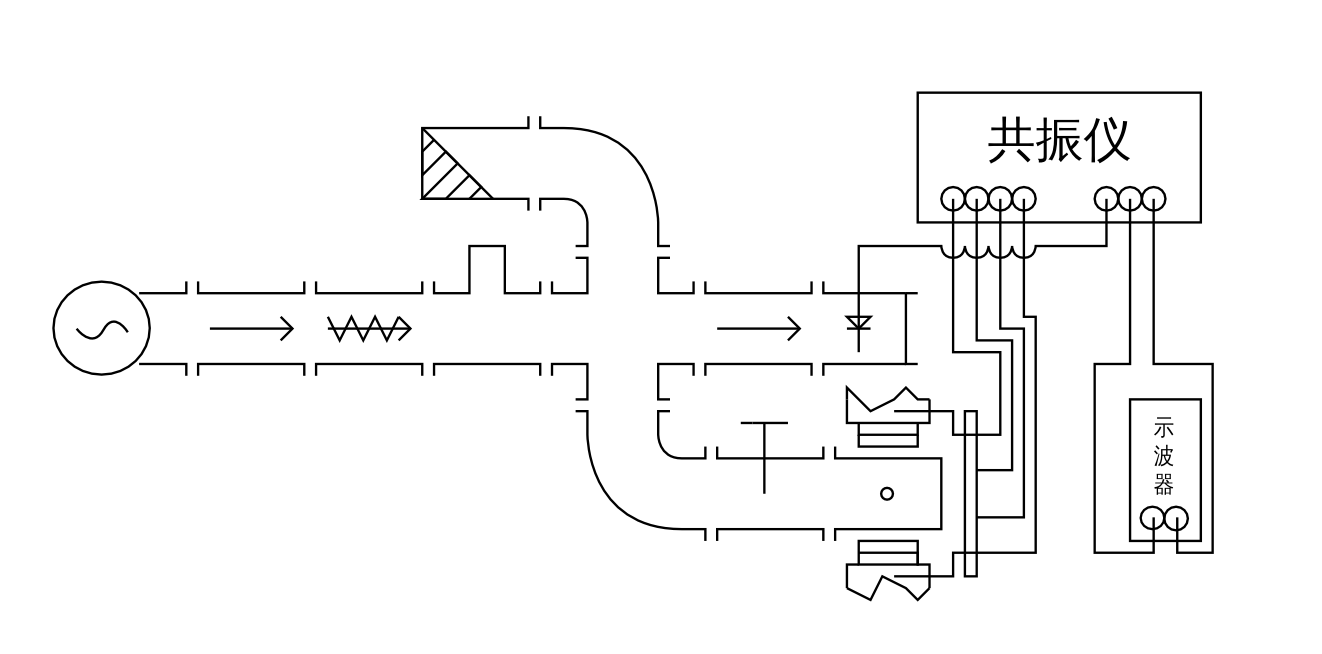
\includegraphics[width=0.8\textwidth]{pic1.png}
		\caption{\label{fig:exp1}利用微波仪器测量DPPH的朗德因子及弛豫时间的实验装置示意图}
	\end{center}
\end{figure}

其中实验装置最左端是一个产生微波的固态信号源,稳定的产生固定频率(8330MHz)的TE10电磁波,微波信号由信号源的体效应振荡器产生并可以调整其频率。微波在TE10波导管中传播,经过隔离器,衰减器,波长计进入双T接头(魔T)的H端。其中隔离器的作用是为了防止后端设备对固态源的影响,而波长计则是准确的测量管中微波的波长。在不进行波长测量的时候应该对波长计进行失谐处理而避免其影响整个微波回路。

微波信号经过魔T分别进入图示中上端和下端的负载。在合理的调节两个负载的阻抗并使之匹配之后,微波在桥路中平衡形成驻波。由麦克斯韦方程组结合魔T的边界条件可知,这时候微波不会向魔T的E端传播,所以此时E端的检波晶体就不会检测到微波信号。

魔T两侧的两臂上的一端中放有样品。未加外界磁场的时候调节调配器使得魔T平衡,而当加入合适的磁场时候,样品吸收微波形成共振,这时候改变了样品所在臂的阻抗,从而阻抗不再匹配。这样的话就可以通过检波晶体观测到顺磁共振的现象了。

\subsection{实验步骤以及数据}

首先根据仪器的属性将固态源的频率调整到一个合适的频率,放开衰减器,使得微波进入后续的谐振组件,并在检波器上观测到示数。因为魔T的一臂已经被调整到了合适的阻抗并对微波进行完全的吸收,所以只需要合理的调整含有样品的一臂的调节器,使得阻抗匹配后就可以观测到检波电流衰减到接近于0。

因为调整器用有两个自由度,所以需要细致的调节衰减器的位置,使得在衰减器基本无衰减,检波器放大倍数足够大的情况下依然得到接近于0的数值。具体的调整方式会在分析讨论中阐述。

当检波器检测不到信号的时候表明,微波已经在魔T的两臂形成了共振吸收,此时微波的频率即是带测样品臂的谐振频率。这时候通过将电磁铁通上约0.32T的稳恒磁场$B_0$,并在电磁场的电流上加上一个扫场电流(0.2-0.7A左右),使得此时的磁场满足一个有0.32T偏置的三角波磁场。如下\ref{fig:exp2}左所示:

\begin{figure}[h]
	\begin{center}
		\subfigure{
			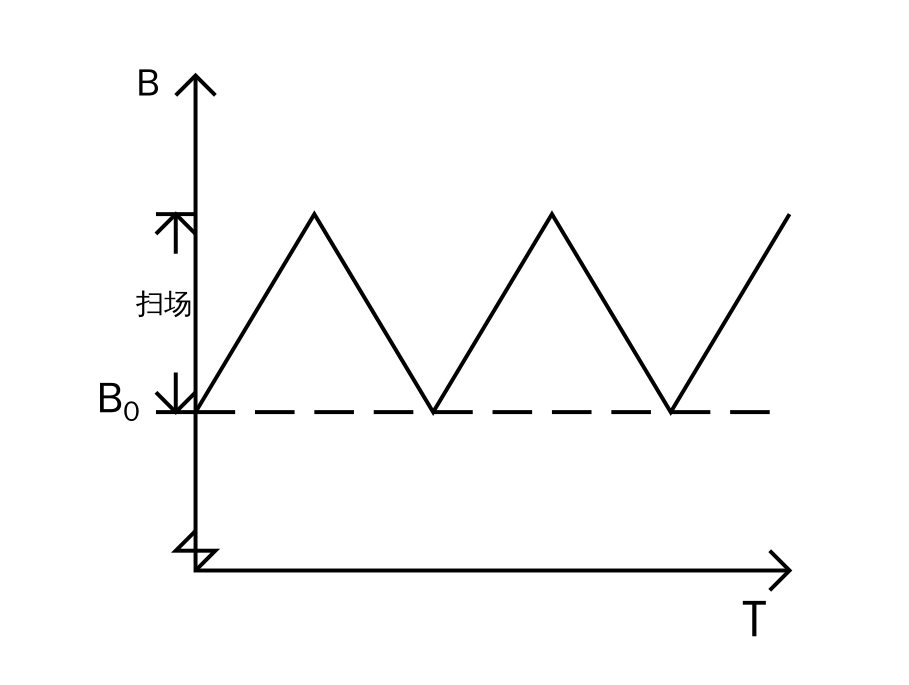
\includegraphics[width=0.4\textwidth]{pic2.png}}
		\subfigure{
			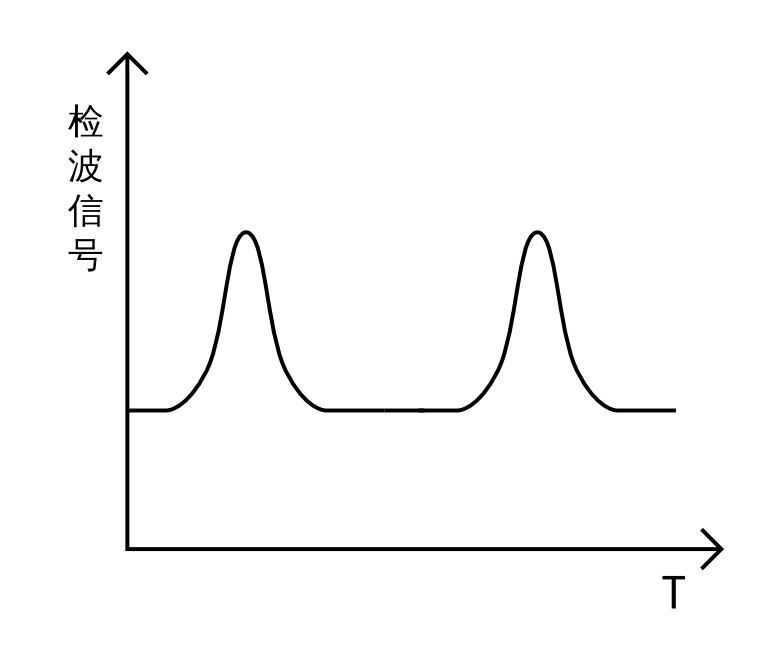
\includegraphics[width=0.4\textwidth]{pic3.png}}
		\caption{\label{fig:exp2}左图:利用微波仪器测量DPPH的朗德因子及弛豫时间的磁场强度随时间的变化图示意图。右图:检波器示数随时间变化示意图。}
	\end{center}
\end{figure}

在以上的调节比较合理的情况下示波器可以得到如\ref{fig:exp2}右图所示的波形。使用X-Y模式观测检测信号和扫场电流可以明显的观测到李萨如图形上有两个波峰。出现波峰的位置即为带测样品达到顺磁共振的位置。

调整稳恒磁场的电流以及扫场电流使得在检测信号随时间变化的波形上两个波峰等间距出现,这时候磁场的平均值就正好是满足电子顺磁共振的磁场强度。利用霍尔元件测量样品附近(正上方)的磁场强度得到的数值为$B=0.3218T$。此时频率计示数为4.606mm,对应的频率为$f=8830MHz$。

经典情况下,电子自旋共振的信号应该是宽度应该是0,即出现一个很窄的吸收线,但实际情况下共振线不是无限窄而是有一定的宽度。这是因为电子在某一个能级上能停留的时间是不确定的,所以根据量子力学不确定性原理有$\delta E \cdot \delta t \sim \hbar$,所以不确定性关系可以写为:
\begin{equation}
	\delta H \cdot \delta t \sim \frac{1}{\lambda}
\end{equation}

在这里线宽可以看做是一个表征驰豫强弱的度量,我们引入一个表征驰豫快慢的物理量——驰豫时间T,其定义为:
$$\Delta H =\frac{1}{\lambda T}$$
式子中的$\Delta H$为线宽。对于稳定的洛伦兹线性自由基,理论上给出:
\begin{equation}
	T_2=\frac{2}{\lambda \Delta H}
\end{equation}

所以说本次实验只要测出线宽就可以确定$T_2$了。测量时将示波器置于X——Y模式,调整相位使得两个波峰重合。此时可以测量出半高宽也就是$\Delta H$所占据的格数。调整磁场的大小,这是屏幕显示的两个波峰会移动,通过测量移动格数和对应的磁场变化即可确定每格对应的磁场大小从而确定$\Delta H$的测量值。这么做的原因会在讨论中予以阐述。

测量得到的数据为半高宽为3.9小格。对应的是不起上每30格磁场强度为2.2mT。此时的频率没有变化依然是$8830MHz$。

\section{数据分析及讨论}

首先是上文中的一些问题和实验中的现象进行解释。首先是对于调整器调节方式的一些现象的研究和分析。因为调节器有纵向和横向两个自由度,所以说检波器的信号强度是两个变量的函数,可以表示为$f=f(x,y)$。而对于二元函数的极值问题,数学上给出一种找到极值点的方法。首先固定y值不变,找出f关于x变量的极小值点,此时这是一个关于x和y的函数$g(x,y)=\frac{\partial f}{\partial y}=0$,然后再在这个函数上找到关于y的极值点,此时就是二元函数$f(x,y)$的极值点。

在实际操作中因为$g(x,y)$往往不是简单的线性函数所以在操作两个两个变量使得函数值取得极值是一件很困难的事情。不过在本次实验中我发现,在确定纵坐标为0.00mm的时候,横坐标取1.6cm时有一个极小值。在纵坐标为5.00mm的时候横坐标取1.1cm有一个极小值,而在纵坐标为2.50mm的时候横坐标去1.4cm有一个极小值。所以可以看出$g(x,y)=0$函数在这个实验中粗略的可以认为是一个线性的函数,所以在满足$x+y\sim 1.6cm$的位置上找极值会更方便一些(这个数值和具体的仪器有关,同时精确的$g(x,y)=0$函数应该由麦克斯韦方程加上隔离器边界条件解出)。

第二个问题就是关于检波器图像以及调节平衡的问题。往往因为调节精度以及仪器自身属性的问题,我们往往并不能严格的通过调整调整器使得检波器的示数为0。接下来就是阐述平衡与否对于实验的具体影响。

理想情况下,魔T两臂应该是严格的平衡的,这时候在外加扫场电流的情况下,检波器所检测的微波信号应该只有在材料发生顺磁共振的时候才会有波峰,否者都会为0。如下图左,而当不是严格平衡的情况下,阻抗本身就不匹配,相当于在本底噪声之上叠加了顺磁共振的波峰。所以出现了如图中和右所示的图形。

\begin{figure}[h]
	\begin{center}
		\subfigure{
			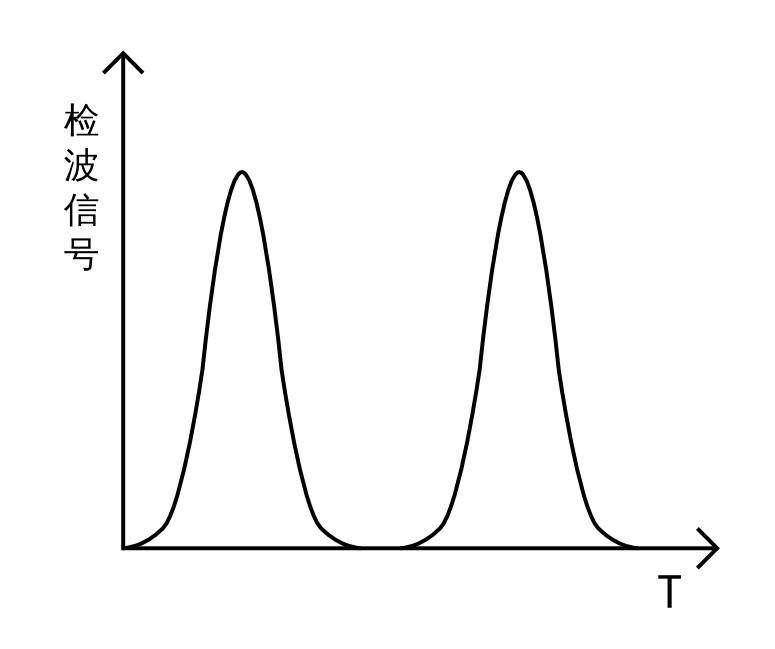
\includegraphics[width=0.3\textwidth]{pic4.png}}
		\subfigure{
			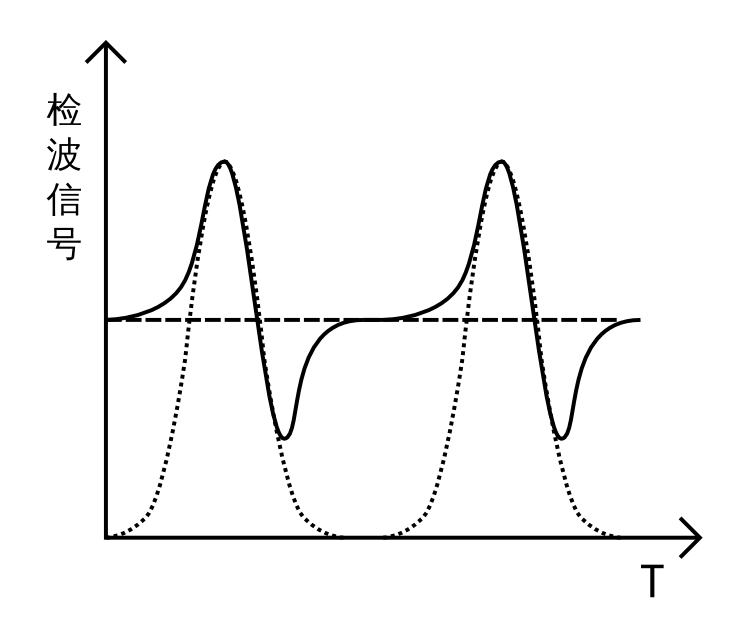
\includegraphics[width=0.3\textwidth]{pic5.png}}
		\subfigure{
			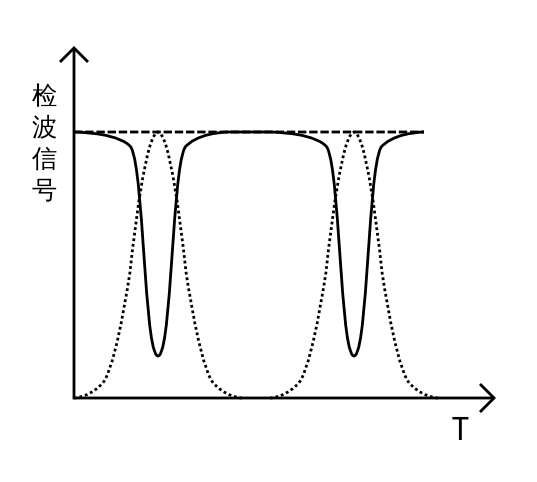
\includegraphics[width=0.3\textwidth]{pic6.png}}
		\caption{\label{fig:exp3}阻抗不匹配时候的检波器信号示意图。}
	\end{center}
\end{figure}

所以从上图可看出,当阻抗不匹配的时候,影响的只有图像的形状和清晰程度,也就是说越不匹配越不容易得到良好的图形,而对实际上的观测测量没有特别巨大的影响。所以说当调节平衡的时候无法做到严格的阻抗匹配其实也可以继续实验下去。不过当阻抗不匹配的时候,并不是一个简单的底噪线性叠加样品共振的信号,这一点我想了好久没有得到一个比较合理的理论解释,有待于进一步的研究。

第三个问题是关于测量$\Delta H$的原理。我们希望测量得到的数据是$\Delta H$,但是利用霍尔元件测量磁场强度只能做到测量稳恒磁场的磁场强度,所以说直接测量扫场磁场变化区域然后按照数格子的方法测量出$\Delta H$是不现实的。而探测信号与磁场强度又有以下关系:

\begin{figure}[h]
	\begin{center}
		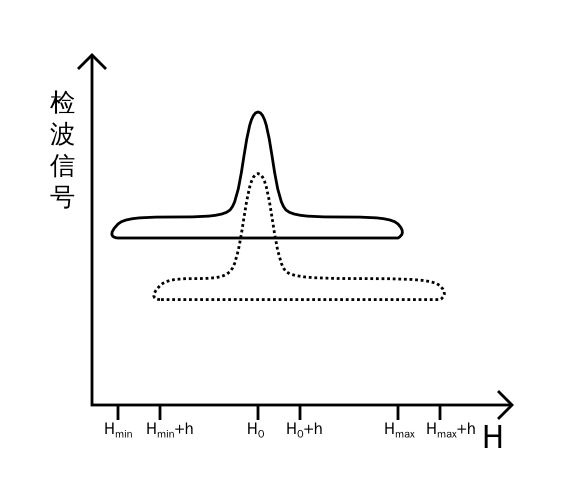
\includegraphics[width=0.6\textwidth]{pic7.png}
	\end{center}
\caption{\label{fig:exp4}探测信号与整体磁场强度的关系示意图。波形表示的是示波器上X——Y通道观测到的波形,垂直方向有移动是为了区别两个波形的不同而刻意移动的,即两个波形的纵坐标应该是一致的。}
\end{figure}

从图片可以看出,当我们在原始的磁场下整体增大磁场强度h后,顺子共振的点沒有移动,而是整体图案向右移动,反映在示波器X——Y通道检测探测信号和扫场强度的图样上就是波峰向左移动。其移动的距离也就代表着磁场变化的大小。这样就可以根据这一点定标出示波器所显示的磁场大小从而得到对应的$\Delta H$。

最后是数据处理部分,将磁场大小和频率带入公式可以得到样品的朗德因子,其数值为$g=1.96$,旋磁比$\gamma=1.72\times 10^{11}$。朗德因子略小于理论数值,我认为偏小的原因有可能是因为在测量磁场强度的时候,使用特斯拉计测量的不是样品位置处的磁场,而更靠近于电磁铁,这样导致测量的磁场偏大从而使g值偏小。而朗德因子测量的误差来源我认为主要是频率计,其精确度为10MHz量级,同时他是测量极小值,所以由测量者引入的主观误差也比较大。

计算得到的驰豫时间为$T_2=4.3\times 10^{-8}$。这个测量的误差我觉得主要来自于对于磁场定标的困难,以及示波器读数的精度问题。想要减少误差我认为可以将定标时多次测量去平均值改为测量不同位置的磁场强度,然后线性回归得到磁场和示波器格子数目的对应关系,这样应该能得到更精确的数据。同时使用读数示波器可以部分的减少因为操作读数带来的的误差。

\section{结论}

这次实验利用的微波器件测量得到了样品DPPH的朗德因子,旋磁比以及驰豫时间:
$$g=1.96$$
$$\gamma=1.72\times 10^{11}$$
$$T_2=4.3\times 10^{-8}$$

测量得到的数据基本和理论预测相一致。

\section{致谢}
感谢王常生老师的指导,以及贾春燕,冉书能老师的技术支持。



\begin{thebibliography}{}
	\bibitem{Book} 吴思成,王祖铨~2010 近代物理实验(第三版)(北京:高等教育出版社)第371页.
%
%
\end{thebibliography}

\clearpage
\appendix
\section{思考题}

\end{document} 
